\section*{Classifier Metrics}
\label{appendix:classifier}

\paragraph{Accuracy}
$$
\text{Accuracy} = \frac{\text{Total Correct Predictions}}{\text{Total Predictions}}
$$

\paragraph{F1-Score}
$$
\text{F1-score} = \frac{2 \times \text{Precision} \times \text{Recall}}{\text{Precision} + \text{Recall}}
$$

\paragraph{Precision}
$$
\text{Precision} = \frac{\text{True Positives}}{\text{True Positives} + \text{False Positives}}
$$

\paragraph{Recall}
$$
\text{Recall} = \frac{\text{True Positives}}{\text{True Positives} + \text{False Negatives}}
$$

\begin{table}[h]
\centering
\caption{Classification Report for Logistic Regression}
\begin{tabular}{lcccc}
\hline
\textbf{Class} & \textbf{Precision} & \textbf{Recall} & \textbf{F1-score} & \textbf{Support} \\
\hline
STOP  & 0.88 & 0.90 & 0.89 & 821 \\
GO    & 0.68 & 0.70 & 0.69 & 821 \\
RIGHT & 0.79 & 0.78 & 0.79 & 821 \\
LEFT  & 0.85 & 0.81 & 0.82 & 821 \\
\hline
\textbf{Accuracy} & \multicolumn{4}{c}{0.80} \\
\textbf{Macro Avg} & 0.80 & 0.80 & 0.80 & 3284 \\
\textbf{Weighted Avg} & 0.80 & 0.80 & 0.80 & 3284 \\
\hline
\end{tabular}
\label{tab:classification_report}
\end{table}


\begin{table}[h]
\centering
\caption{Classification Report for KNN}
\begin{tabular}{lcccc}
\hline
\textbf{Class} & \textbf{Precision} & \textbf{Recall} & \textbf{F1-score} & \textbf{Support} \\
\hline
STOP  & 0.92 & 0.99 & 0.95 & 821 \\
GO    & 0.78 & 0.82 & 0.80 & 821 \\
RIGHT & 0.93 & 0.84 & 0.88 & 821 \\
LEFT  & 0.91 & 0.87 & 0.89 & 821 \\
\hline
\textbf{Accuracy} & \multicolumn{4}{c}{0.88} \\
\textbf{Macro Avg} & 0.88 & 0.88 & 0.88 & 3284 \\
\textbf{Weighted Avg} & 0.88 & 0.88 & 0.88 & 3284 \\
\hline
\end{tabular}
\label{tab:knn_classification_report}
\end{table}


\begin{table}[h]
\centering
\caption{Classification Report for Random Forest}
\begin{tabular}{lcccc}
\hline
\textbf{Class} & \textbf{Precision} & \textbf{Recall} & \textbf{F1-score} & \textbf{Support} \\
\hline
STOP  & 0.93 & 0.98 & 0.95 & 821 \\
GO    & 0.76 & 0.87 & 0.81 & 821 \\
RIGHT & 0.95 & 0.85 & 0.89 & 821 \\
LEFT  & 0.92 & 0.84 & 0.88 & 821 \\
\hline
\textbf{Accuracy} & \multicolumn{4}{c}{0.88 (3284 samples)} \\
\textbf{Macro Avg} & 0.89 & 0.88 & 0.88 & 3284 \\
\textbf{Weighted Avg} & 0.89 & 0.88 & 0.88 & 3284 \\
\hline
\end{tabular}
\label{tab:random_forest_classification_report}
\end{table}


\begin{table}[h]
\centering
\caption{Classification Report for SVM}
\begin{tabular}{lcccc}
\hline
\textbf{Class} & \textbf{Precision} & \textbf{Recall} & \textbf{F1-score} & \textbf{Support} \\
\hline
STOP  & 0.90 & 0.96 & 0.93 & 821 \\
GO    & 0.79 & 0.82 & 0.81 & 821 \\
RIGHT & 0.92 & 0.88 & 0.90 & 821 \\
LEFT  & 0.95 & 0.89 & 0.92 & 821 \\
\hline
\textbf{Accuracy} & \multicolumn{4}{c}{0.89 (3284 samples)} \\
\textbf{Macro Avg} & 0.89 & 0.89 & 0.89 & 3284 \\
\textbf{Weighted Avg} & 0.89 & 0.89 & 0.89 & 3284 \\
\hline
\end{tabular}
\label{tab:svm_classification_report}
\end{table}



\clearpage
\section*{User Study Web Interface} \label{app:web_interface}

\vspace{-0.75em}
\noindent
This section shows the screenshot of the web interface used in the user evaluation study (see Section~\ref{subsubsec:quantitative_analysis_of_user_ratings} for the explanation flow).

\vspace{-0.5em}

\begin{figure}[h]
    \centering
    \captionsetup{font=small,skip=4pt}
    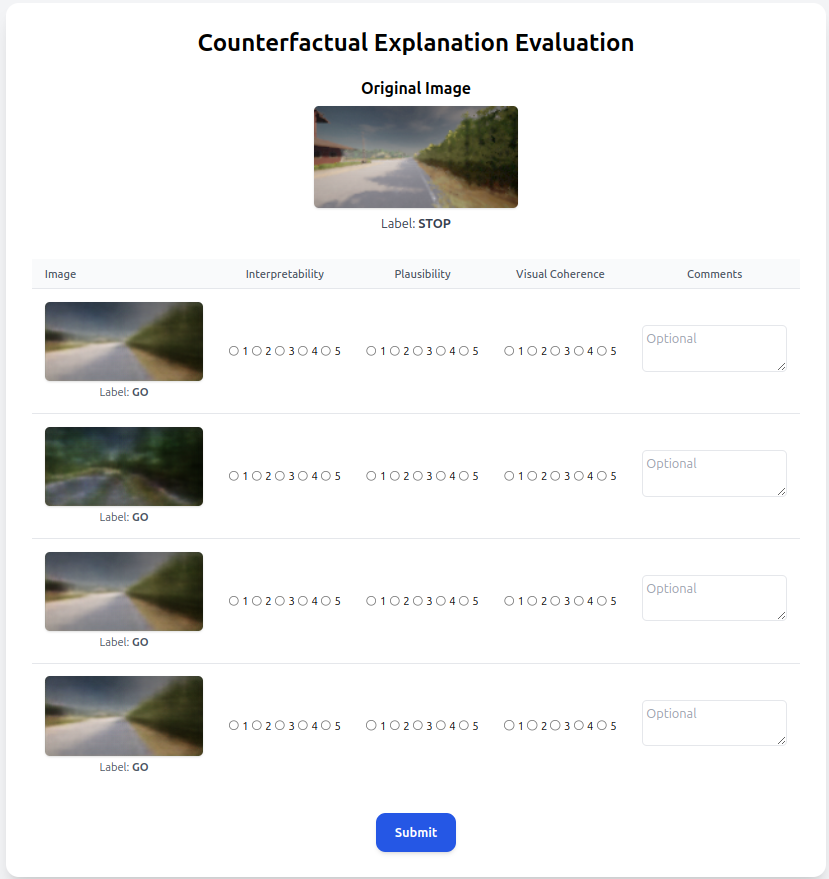
\includegraphics[width=0.68\textwidth]{img/web_app_screenshots/grading.png}
    \caption{Screenshot of the web-based evaluation interface developed for the human user study. The interface presents the original driving scene image (with its predicted label, in this case, \texttt{STOP}) at the top, followed by four counterfactual images—each assigned a predicted label (e.g., \texttt{GO}). For each counterfactual, participants rate interpretability, plausibility, and visual coherence on a 5-point Likert scale. Optional comment boxes are provided for qualitative feedback. This interface implementation is discussed in Section~\ref{subsubsec:quantitative_analysis_of_user_ratings}.}
    \label{fig:app:grading}
\end{figure}


\begin{sidewaysfigure}[htbp]
    \centering
    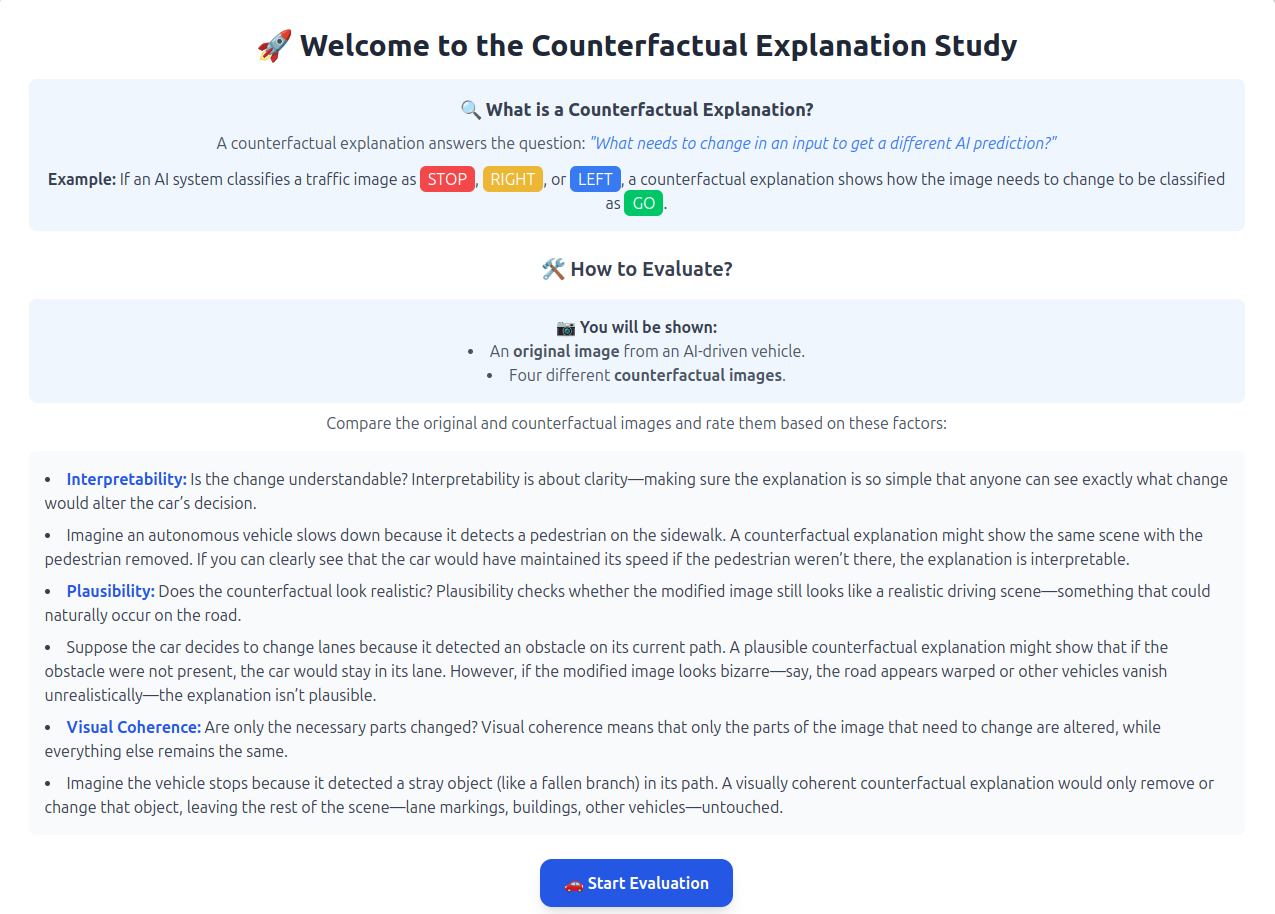
\includegraphics[width=0.78\textwidth]{img/web_app_screenshots/form_ui_info.png}
    \caption{Welcome screen of the user evaluation interface used in the counterfactual explanation study. This introductory page provides participants with a concise overview of the purpose of counterfactual explanations in the context of traffic scene classification (e.g., changing an image classified as \texttt{STOP} to \texttt{GO}). It explains what participants will be shown (an original image followed by four counterfactuals) and outlines the evaluation criteria: Interpretability, Plausibility, and Visual Coherence. Each criterion is defined with examples to ensure a clear and consistent understanding among all evaluators before proceeding to the actual rating task.}
    \label{fig:app:form_ui}
\end{sidewaysfigure}




\clearpage
\section*{Visual Comparison of Successful and Failed Counterfactuals} \label{app:visual_comparasions_of_CE}


\subsection{Examples where Counterfactuals were Successfully Generated}


\begin{figure}[htbp]
\centering
\begin{tabular}{c|ccc}
\textbf{Input Image} 
& \textbf{Grid Based Masking} 
& \textbf{Object Detection Masking} 
& \textbf{LIME on Image Masking} \\
% Row 1: Masked Inputs
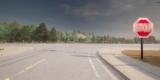
\includegraphics[width=0.18\textwidth]{img/appendix/original_town7_000980.png}
& 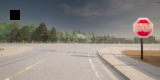
\includegraphics[width=0.18\textwidth]{img/appendix/grid_masked_town7_000980.png}
& 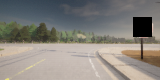
\includegraphics[width=0.18\textwidth]{img/appendix/object_masked_town7_000980.png}
& 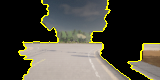
\includegraphics[width=0.18\textwidth]{img/appendix/LIME_on_Image_maksed_town7_000980.png} \\
& \multicolumn{3}{c}{\textcolor{red}{\textbf{STOP Prediction}}} \\
% Row 2 Label
& \multicolumn{3}{c}{\textbf{Corresponding Counterfactual Generated Images}} \\
% Row 3: Counterfactual Reconstructions
& 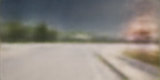
\includegraphics[width=0.18\textwidth]{img/appendix/grid_reconstructed_town7_000980.png}
& 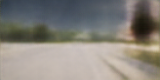
\includegraphics[width=0.18\textwidth]{img/appendix/object_reconstructed_town7_000980.png}
& 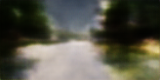
\includegraphics[width=0.18\textwidth]{img/appendix/LIME_on_Image_reconstructed_town7_000980.png} \\
& \textcolor{green}{\textbf{GO}} 
& \textcolor{green}{\textbf{GO}} 
& \textcolor{blue}{\textbf{RIGHT}}
\end{tabular}

\caption{The original image is labeled as STOP. All three masking methods (Grid, Object Detection, LIME on Image) successfully generated counterfactuals. The reconstructions led to new predictions: GO (for Grid/Object) and RIGHT (for LIME Image).}
\label{fig:ce_grid_object_lime}
\end{figure}





